\subsection{Direkte Evaluation der Erklärungen}
\label{sec:study_results_qualitativ}

Die zuvor analysierten Metriken betreffen ausschließlich die Auswirkungen von Erklärungen auf die Qualitäsziele von Graphmasters für die Integration - im konkreten Fall \textit{Usage Increase}, \textit{System Acceptance} und \textit{Satisfaction}. Um einen besseren Überblick über andere Qualitätsaspekte der Erklärungen zu bekommen, erfolgte noch eine direkte Evaluation der Erklärungen.

\subsubsection{Ziel der direkten Evaluation}

Mithilfe der Metriken konnte überprüft werden, welche Erklärungen, in welchen Kombinationen den zuvor aufgestellten Anforderungen genügen. Es kann allerdings für die statischen Erklärungen keine Empfehlung abgeleitet werden, da diese keine signifikant positiven Auswirkungen haben.
% und warum sowohl positive und negative Effekte im Vergleich zum ausschließlichen Einsatz der \textit{Context}-Erklärungen messbar sind.
Folglich ist die direkte Evaluation der Erklärungen nötig, wie sie auch im Leitfaden vorgeschlagen wird. Insbesondere wird dort empfohlen nicht nur Verhaltensmetriken, sondern auch qualitative Evaluationen von \textit{End Usern} zur Bewertung von Erklärungen zu nutzen. Daher ist im Anschluss an die \textit{Case Study} ein Quasi-Experiment mit vier Nutzern durch durchgeführt worden. Diese zweite Analyse sollte zusätzliche Daten liefern, um die Ergebnisse Einflüsse der integrierten Erklärungen auf andere Qualitätsaspekte besser interpretieren zu können.

Das Ziel ist es folglich, konkrete Probleme oder Verbesserungspotential der entwickelten Erklärungen aufzudecken und somit fehlende positive Effekte aus der \textit{Case Study} zu erklären.

\subsubsection{Methode}

Die direkte Analyse der Erklärungen ist wiederum in zwei Teile gegliedert. Zum einen wurden während der \textit{Case Study} einige Meta-Daten gesammelt. Es wurde beispielsweise aufgezeichnet, wie viele der \textit{End User}, die die Möglichkeit hatten, auf die statischen Erklärungen zuzugreifen, diese genutzt haben und wie lange, sie diese im Fokus hatten.

Um qualitative Aussagen zu den Erklärungen zu erhalten wurde daher ein Quasi-Experiment durchgeführt. Bei diesem wurde vier Studienteilnehmern jeweils alle vier Erklärungen gezeigt bzw. sie sollten mit diesen interagieren. Im Anschluss an jede Erklärung wurden ihnen die gleichen Aussagen zur Bewertung auf einer Likert-Skala vorgelegt. Diese entsprechen den im Leitfaden unter Evaluation vorgestellten Aussagen (siehe \autoref{sec:model_evaluation}). Das heißt mithilfe der Aussagen zu den Erklärungen werden die Qualitätsaspekte \textit{Satisfaction}, \textit{Perceived Transparency}, \textit{Persuasiveness}, \textit{Usefulness} und \textit{Completeness} der Erklärungen bewertet. Darüber hinaus wurden Aussagen zum \textit{Demand} der jeweiligen Erklärung hinzugefügt.

Außerdem wurden die Teilnehmer gebeten, alle Gedanken beim Interagieren oder Lesen der Erklärungen mitzuteilen (\textit{Think-Aloud}-Experiment). Anschließend an jede Erklärung haben alle Teilnehmer außerdem die Möglichkeit erhalten, Verbesserungsvorschläge für die Erklärungen zu machen oder auf fehlende Informationen in der Erklärung hinzuweisen. Der vollständige Fragebogen mit dem Ablauf des Quasi-Experiments ist in \nameref{ch:appendix_1} zu finden.

Teilgenommen haben insgesamt drei Männer und eine Frau im Alter von 23 - 55 Jahren. Alle Nutzer waren mit Navigationsanwendungen wie Google oder Apple Maps vertraut und drei der vier Teilnehmer nutzen Navigationsanwendungen regelmäßig. Zwei der Teilnehmer haben außerdem sehr viel Erfahrung mit \textit{NUNAV Navigation} (<10 mal benutzt), einem Teilnehmer war die Anwendung bekannt (2-3 mal verwendet) und eine Teilnehmerin hat die Anwendung noch nicht verwendet gehabt (siehe \nameref{ch:appendix_1}). Jeweils eine Person der Teilnehmergruppe passte zum Großteil auf eines der beiden vorgestellten Personas.

Im Folgenden werden die Ergebnisse der direkten Evaluation der Erklärungen vorgestellt.

\subsubsection{Bedarf für die gegebenen Erklärungen}
\label{sec:demand_qualitative_evaluation}

Die statischen Erklärungen (siehe \autoref{sec:explanation_design}), welche die Einflüsse auf den Routing-Algorithmus von NUNAV sowie das kollaborative Routing erklären, sind interaktiv. Somit kann evaluiert werden, wie viele Studienteilnehmer der \textit{Case Study} diese wie häufig diese angefordert haben. Außerdem kann gemessen werden, wie lange sie die Erklärungen betrachtet haben. Die Studiengruppen, denen diese angezeigt wurden (Gruppe 2 und 4), enthielten insgesamt 1~766 Teilnehmer.

Als erfasst und nicht direkt wieder verlassen werden die Erklärungen gewertet, wenn die \textit{End User} länger als 1,5 Sekunden in dem Dialog verbracht haben \cite{BAHR2011776}. So können die Daten herausgefiltert werden, bei denen \textit{End User} versehentlich den Dialog aufgerufen haben. \autoref{fig:explanation_results_clicked} zeigt die Häufigkeit der Aufrufe für die beiden Erklärungstypen. \autoref{fig:01_collaborative_routing_demand} und \autoref{fig:02_collaborative_algorithm_demand} zeigen die Bewertung der Studienteilnehmer des Quasi-Experiments in Bezug auf deren Bedarf für die Erklärungen.

\begin{figure}[htb!]
    \centering
    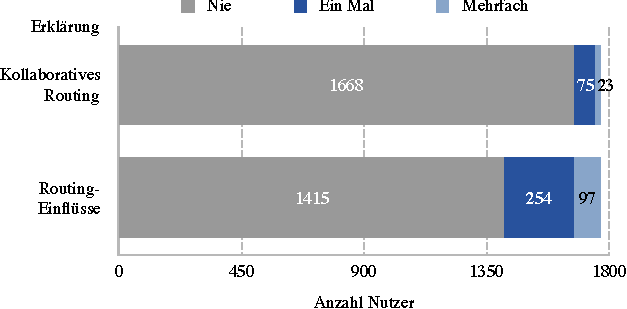
\includegraphics[width=0.9\textwidth]{contents/06_model_evaluation/02_evaluation/res/explanation_results_clicked.pdf}
    \caption{Häufigkeit der Aufrufe der Erklärungen zum Routing-Algorithmus sowie dessen äußeren Einflüssen}
    \label{fig:explanation_results_clicked}
\end{figure}

In der \autoref{fig:explanation_results_clicked} kann man erkennen, dass etwa 5~\% der Nutzer auf die Erklärung zum kollaborativen Routing geklickt haben. Allerdings sagen wie in \autoref{fig:01_collaborative_routing_demand} zu erkennen ist, drei von vier Teilnehmern des Quasi-Experiments, dass sie die Erklärung benötigt haben. Folglich herrscht eine Diskrepanz zwischen dem wirklichen Bedarf und den \textit{End Usern} der \textit{Case Study}, die die Erklärung angefordert haben. Insbesondere haben im Quasi-Experiment zwei der Teilnehmer angegeben, die Erklärung sich auch mehrfach anzusehen. Nichtsdestotrotz gegeben zwei Teilnehmer an, die beiden Erklärungstypen ausblenden können zu wollen.

\begin{figure}[htb!]
    \centering
    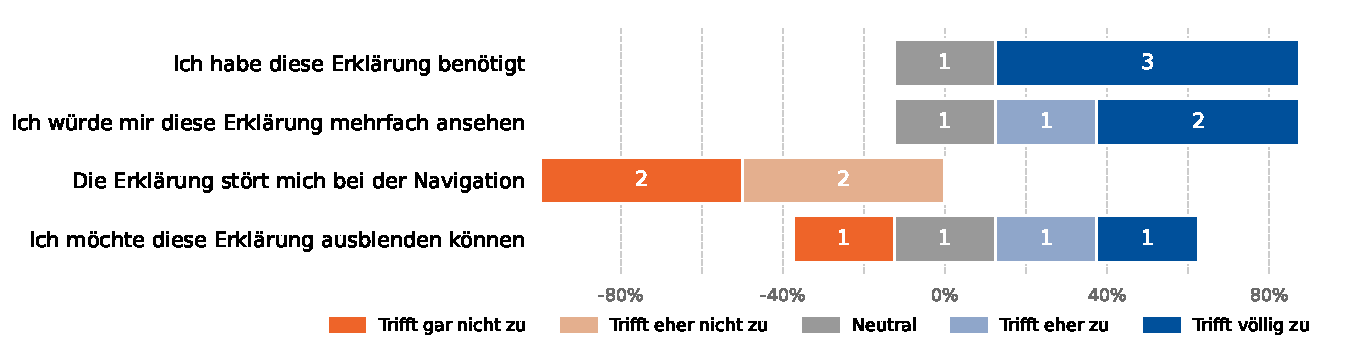
\includegraphics[width=\textwidth]{contents/06_model_evaluation/02_evaluation/res/qualitativeFeedback-01_collaborative_routing_demand.pdf}
    \caption{Subjektive Einschätzung des Bedarfs für die Erklärung zum kollaborativen Routing}
    \label{fig:01_collaborative_routing_demand}
\end{figure}

Betrachtet man im Gegensatz dazu die gleichen Daten für die Erklärung zu den Einflüssen auf die Routenberechnung fällt auf, dass etwa 20~\% der Teilnehmer der \textit{Case Study} sich die Erklärung angesehen haben. Wie in \autoref{fig:02_collaborative_algorithm_demand} allerdings zu sehen ist, haben sowohl weniger Teilnehmer angegeben, dass sie die Erklärung benötigt haben, als auch sich mehrfach ansehen würden als bei der Erklärung zum kollaborativen Routing. Ein Erklärungsversuch kann durch die Aussage eines Teilnehmers am Quasi-Experiment getätigt werden. Dieser sagte, dass die Zahl, auf die für die kollaborative Routing Erklärung geklickt werden müsse, zum Teil klar ist und nicht direkt offensichtlich ist, dass sich dort hinter die Erklärung befinde. Außerdem hat eine Teilnehmerin hinzugefügt, dass die Frage \glqq Wie ist meine Route entstanden?\grqq{}, über welche die Erklärung zu den Routing-Einflüssen erreichbar ist, neugieriger macht, als die angezeigte Zahl der aktiven Nutzer in der Nähe.

\begin{figure}[htb!]
    \centering
    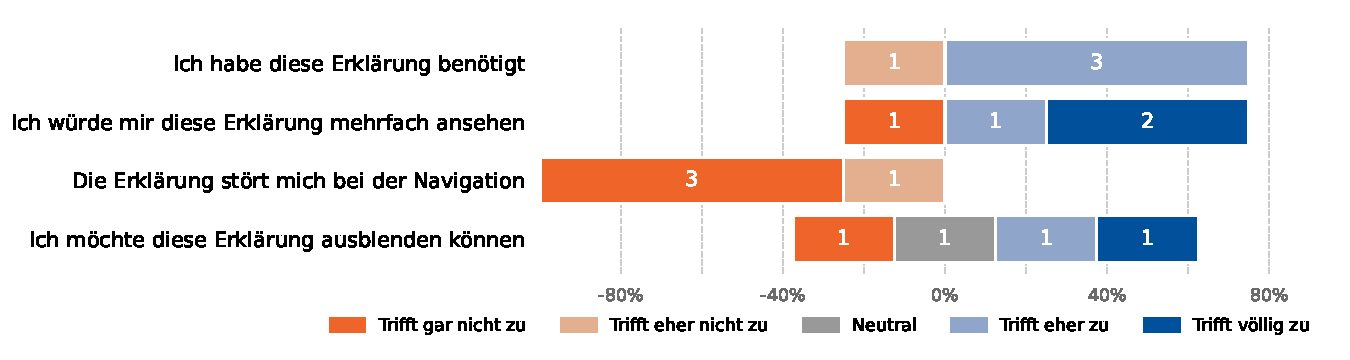
\includegraphics[width=\textwidth]{contents/06_model_evaluation/02_evaluation/res/qualitativeFeedback-02_collaborative_algorithm_demand.pdf}
    \caption{Subjektive Einschätzung des Bedarfs für die Erklärung zu Einflüssen auf den Routingalgorithmus}
    \label{fig:02_collaborative_algorithm_demand}
\end{figure}

Aus diesen freien Aussagen und dem Gegensatz zwischen den benötigten Erklärungen und den wirklich angeforderten, kann folglich abgeleitet werden, dass die Erklärung zum kollaborativen Routing offensichtlicher zu erreichen sein sollte. Die Idee eines weiteren Teilnehmers war, dass es Möglich sein sollte, diese Erklärung über den Dialog \glqq Trete Schwarm bei...\grqq{} erreichen zu können. Dies ist der Dialog, der zu sehen ist, während \textit{NUNAV Navigation} die erste Route während der Nutzung lädt. Er hat außerdem hinzugefügt, dass an dieser Stelle der Schwarmbegriff unverständlich sei und durch die Erklärung klar würde.

Außerdem kann es dadurch, dass nur bis zu 20~\% der \textit{End User} in der \textit{Case Study} die Erklärungen gelesen haben, sein, dass die Auswirkungen auf andere Qualitätsmerkmale in der Studie nicht im signifikanten Bereich lagen. Zumindest für die Erklärung zum kollaborativen Routing ließe sich dies anhand der Aussagen der Teilnehmer des Quasi-Experiments durch einen verbesserten Weg, um zur Erklärung zu gelangen, ggf. steigern und sollte in einer zweiten Iteration getestet werden. Des Weiteren gab es in einem Fall beim Quasi-Experiment Kritik daran, dass die Hilfe-Center-Artikel im Browser des Smartphones geöffnet würden. Eine Integration in der App würde der Aussage nach eher dazu bewegen, sich eine Erklärung auch durchzulesen.

Für die beiden \textit{Context-Abhängigen} Erklärungen gab es keine Metriken, welchen den Bedarf innerhalb der \textit{Case Study} widerspiegeln können. Auch gab es im Rahmen des Quasi-Experiments lediglich positive Rückmeldungen zum Bedarf der Erklärungen. Des Weiteren wurden beide Erklärungen weder als störend empfunden, noch gab es Studienteilnehmer, die den Wunsch äußerten, die Erklärungen ausblenden zu wollen (siehe \autoref{fig:03_traffic_volume_demand} und \autoref{fig:04_position_accuracy_demand}). Außerdem gab es auch keine weiteren Äußerungen der Teilnehmer des Quasi-Experiments zu den beiden Erklärungen. Daher können aus den Daten zum Bedarf für diese Erklärungen keine Verbesserungsmöglichkeiten abgeleitet werden. Dies deckt sich mit den positiven Ergebnissen aus der \textit{Case Study}.

\begin{figure}[htb!]
    \centering
    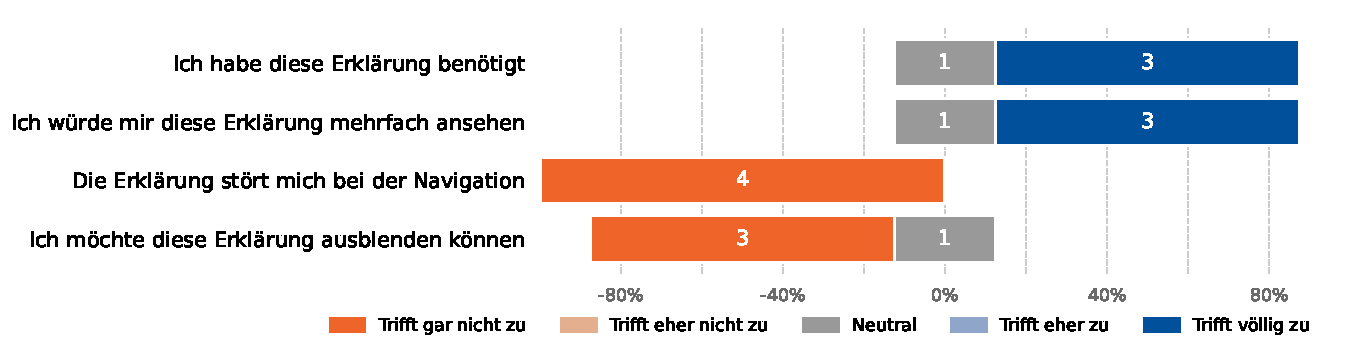
\includegraphics[width=\textwidth]{contents/06_model_evaluation/02_evaluation/res/qualitativeFeedback-03_traffic_volume_demand.pdf}
    \caption{Subjektive Einschätzung des Bedarfs für die Erklärung zum aktuellen Verkehrsgeschehen}
    \label{fig:03_traffic_volume_demand}
\end{figure}

\begin{figure}[htb!]
    \centering
    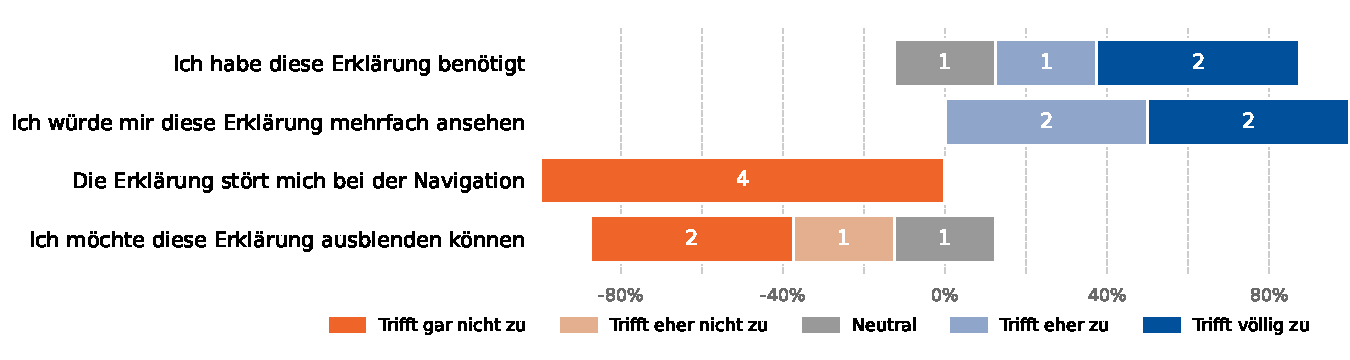
\includegraphics[width=\textwidth]{contents/06_model_evaluation/02_evaluation/res/qualitativeFeedback-04_position_accuracy_demand.pdf}
    \caption{Subjektive Einschätzung des Bedarfs für die Erklärung zu Positionsungenauigkeiten}
    \label{fig:04_position_accuracy_demand}
\end{figure}

\subsubsection{Inhalt der gegebenen Erklärungen}

Um den Inhalt der entwickelten Erklärungen zu bewerten, kann vor allem die \textit{Usefulness}, die \textit{Perceived Transparency} und die \textit{Completeness} der Erklärungen analysiert werden.

Für die beiden statischen Erklärungen kann indirekt die \textit{Usefulness} der Erklärungen im Rahmen der \textit{Case Study} bestimmt werden. Der Hilfe-Center, welche zur Anzeige der Erklärungen genutzt wurde, enthält am Ende jedes Artikel die Möglichkeit, diesen als \glqq Hilfreich\grqq{} oder \glqq Nicht hilfreich\grqq{} zu bewerten. Auf den Hilfe-Center können \textit{End User} zwar auch über andere Wege, als die in der \textit{Case Study} bereitgestellten gelangen. Da es hier allerdings um die Bewertung der Erklärung an sich geht, können die Daten hier nichtsdestotrotz verwendet werden. \autoref{tab:explanation_results_clicked} zeigt die Bewertungen als \glqq Hilfreich\grqq{} oder \glqq Nicht hilfreich\grqq{} für die beiden statischen Erklärungen an.

\begin{table}[htb!]
    \centering
    \begin{tabular}{p{.5\textwidth}p{.15\textwidth}p{.25\textwidth}}
        \hline
        Artikel & Hilfreich & Nicht Hilfreich \\
        \toprule
        Kollaboratives Routing & 76 & 9 \\
        Einflüsse auf die Routenberechnung & 209 & 32 \\
        \bottomrule
    \end{tabular}
    \caption{\textit{Usefulness} der Hilfe-Center-Artikel}
    \label{tab:explanation_results_clicked}
\end{table}

An den Bewertungen, welche aus dem Hilfe-Center stammen, kann man erkennen, dass ein Großteil (90~\% kollaboratives Routing, 87~\% Routing-Einflüsse) der \textit{End User}, welche die Artikel bewertet haben, diese als \glqq hilfreich\grqq{} bewertet haben. Dies spiegelt sich auch in der subjektiven Bewertung der Erklärungen im Quasi-Experiment wider. Mit einer Ausnahme stehen die Studienteilnehmer den Aussagen, dass die Erklärungen nützlich sind und diese verstanden haben positiv oder neutral gegenüber (siehe \autoref{fig:01_collaborative_routing_content} und \autoref{fig:02_collaborative_algorithm_content}). Lediglich ein Teilnehmer hat die Aussage, dass die Erklärung zum kollaborativen Routing nützlich für die Navigation ist mit \glqq Trifft eher nicht zu\grqq{} bewertet. Auf Nachfrage, liegt dies daran, dass der Teilnehmer sich wünschen würde zu sehen, wann das kollaborative Routing ihn direkt während der Navigation beeinflusst. Folglich wird eine weitere \textit{Context}-abhängige Erklärung zusätzlich zur Anzahl der \textit{End User} in der Umgebung benötigt, welche diesen Umstand stärker herausstellt. Die Umsetzung ist aufgrund der benötigten Daten allerdings schwierig.

\begin{figure}[htb!]
    \centering
    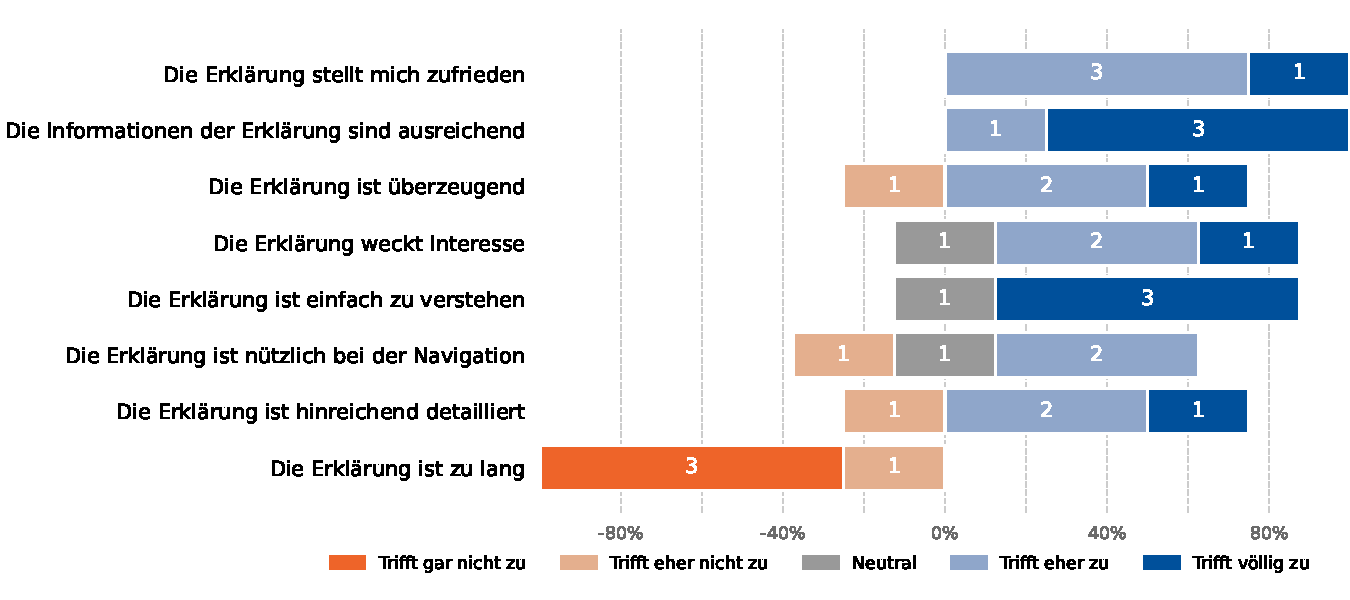
\includegraphics[width=\textwidth]{contents/06_model_evaluation/02_evaluation/res/qualitativeFeedback-01_collaborative_routing_content.pdf}
    \caption{Subjektive Einschätzung des Inhalts für die Erklärung zum kollaborativen Routing}
    \label{fig:01_collaborative_routing_content}
\end{figure}

Bei der Betrachtung von \textit{Perceived Transparency} und \textit{Completeness} sind die Bewertungen für die statischen Erklärungen im Quasi-Experiment überwiegend positiv oder neutral (siehe \autoref{fig:01_collaborative_routing_content}). Eine Aussage zur Erklärung zum kollaborativen Routing, die wiederum negativ beantwortet wurde, stammt von selbigem Nutzer wie zuvor und ist auch ähnlich begründet. Außerdem wurde die Aussage zur Länge der Erklärung zu den Einflüssen auf die Routenberechnung in einem Fall als zu lang bewertet. Die Teilnehmerin hätte sich Formulierungen gewünscht, die etwas schneller das Kernthema erfassen.

\begin{figure}[htb!]
    \centering
    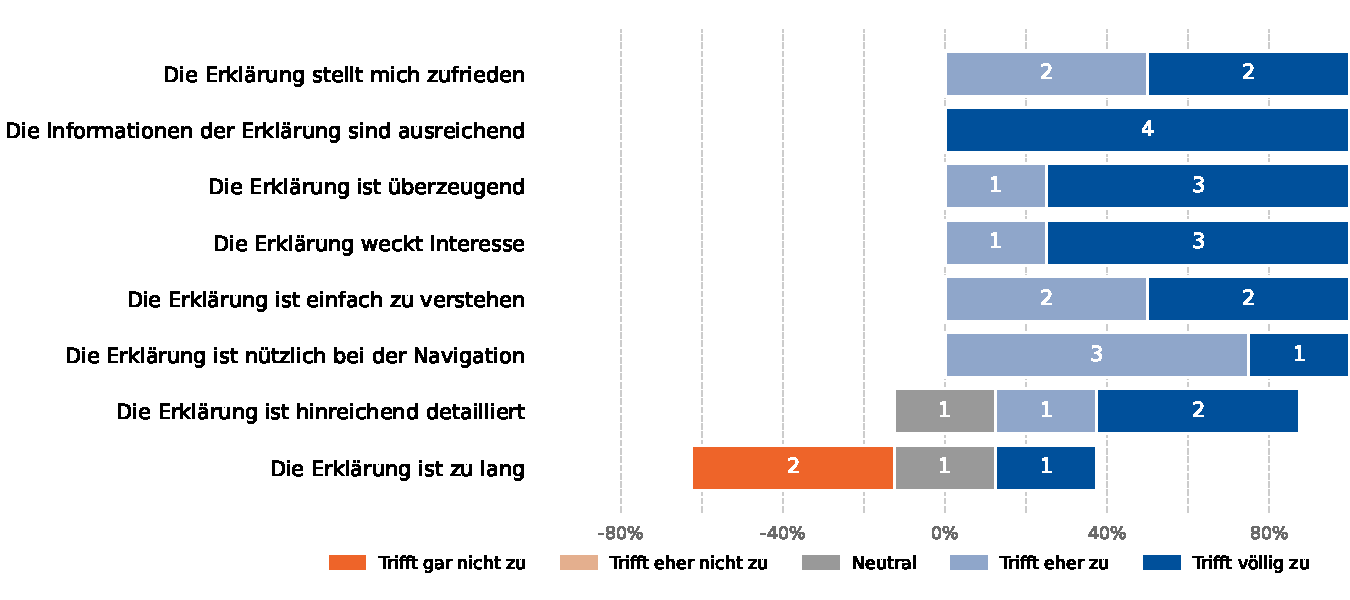
\includegraphics[width=\textwidth]{contents/06_model_evaluation/02_evaluation/res/qualitativeFeedback-02_collaborative_algorithm_content.pdf}
    \caption{Subjektive Einschätzung des Inhalts für die Erklärung zu Einflüssen auf den Routingalgorithmus}
    \label{fig:02_collaborative_algorithm_content}
\end{figure}

Was sich zwar in den Bewertungen der Aussagen nicht widerspigelt, allerdings im offenen Teil des Quasi-Experiments in einem Fall erwähnt wurde, ist, dass sich der Teilnehmer zu den einzelnen Einflüssen auf die Routenberechnung gewünscht hätte, zu sehen, aus welchen Quellen die Daten stammen, um deren Güte zu bewerten.

Zusammenfassend kann für den Inhalt der statischen Erklärungen gesagt werden, dass dieser im Allgemeinen wenig Kritikpunkte im Quasi-Experiment erfahren hat und lediglich an einzelnen Stellen verbesserungswürdig (z.B. in den Formulierungen) ist. Die Forderung nach der Preisgabe der Datenquellen für die Einflüsse auf das Routing ist aufgrund von Verträgen zum Großteil nicht möglich. 

\bigskip

Da die Bewertungen der Aussagen zu den beiden \textit{Context}-abhängigen Erklärungen deutlich unterschiedlich ausfallen, werden diese getrennt behandelt. Für die Erklärung zum aktuellen Verkehrsgeschehen kann gesagt werden, dass der Inhalt ausschließlich positiv bewertet wurde (siehe \autoref{fig:03_traffic_volume_content}). Darüber hinaus sind zusätzlich zu den Bewertungen der vorgegebenen Aussagen weitere positive Kommentare gemacht worden. Dies betrifft beispielsweise Konkurrenzprodukte, welche bereits ähnliche Erklärungen liefern und die Erklärungen zum Verkehrsaufkommen, daher aufgrund der Bekanntheit und guten Erfahrung mit der Funktion als positiv gesehen wird. Folglich muss an der Erklärung an sich aufbauend auf der vorliegenden Analyse nicht verändert werden.

\begin{figure}[htb!]
    \centering
    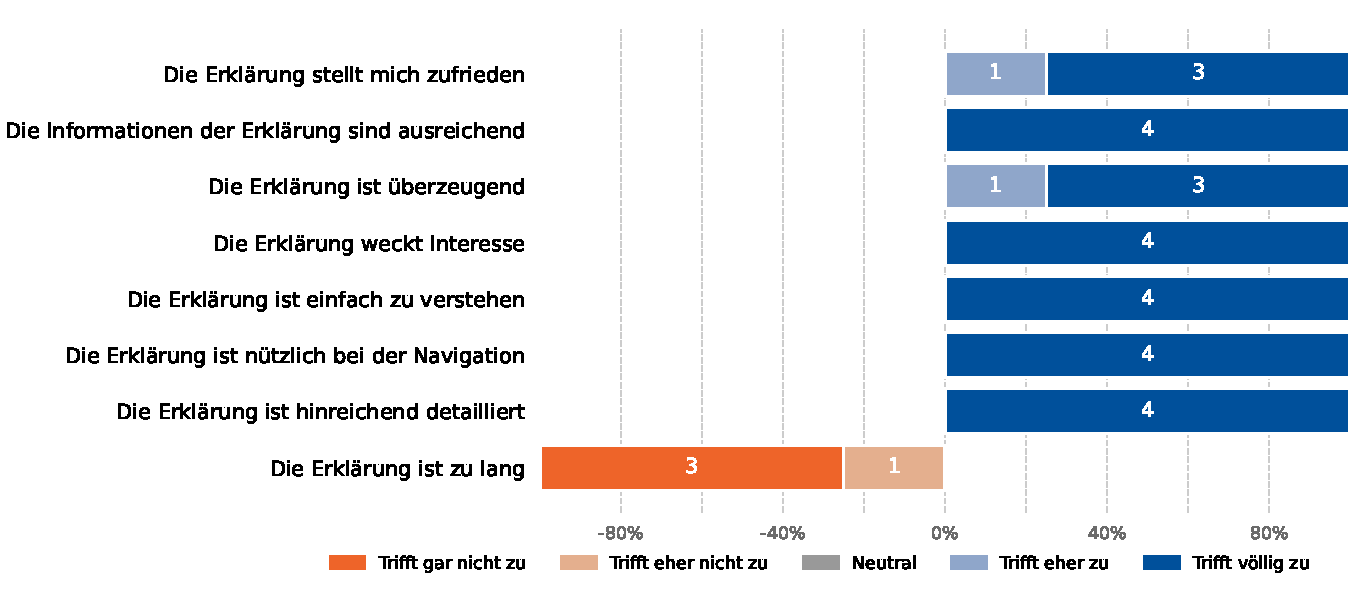
\includegraphics[width=\textwidth]{contents/06_model_evaluation/02_evaluation/res/qualitativeFeedback-03_traffic_volume_content.pdf}
    \caption{Subjektive Einschätzung des Inhalts für die Erklärung zum aktuellen Verkehrsgeschehen}
    \label{fig:03_traffic_volume_content}
\end{figure}

% Betrachtet man allerdings die \textit{Context}-Daten, auf welche die Erklärung aufbaut, so hat der Berechnungsalgorithmus aus den intern  bei Graphmasters gemacht Erfahrungen heraus Verbesserungspotential. Beispielsweise müsste eine Evaluation erfolgen, wie \textit{End User} Verkehr einschätzen und wie oft und wie lange Verkehr auf einer Route beispielsweise subjektiv anders als \glqq normal\grqq{} wahrgenommen werden muss, damit sich dies auf die Wahrnehmung für die ganze Route auswirkt.

\bigskip

Die Erklärung zur ungenauen Positionierung hat, wie in \autoref{fig:04_position_accuracy_content} zu erkennen ist, einzelne negative Bewertungen bezüglich der \textit{Satisfaction} und \textit{Perceived Transparency}. Dies ist darauf zurückführen, dass zwei Teilnehmerinnen bzw. Teilnehmer versucht hatten, über das \textit{Growl}, der zur Erklärung gehört eine genaue Erklärung der Funktion anzufordern und diese nicht erhalten konnten. Dies wurde mit der Frage danach verbunden, was \glqq Position ungenau\grqq{} genau bedeutet. Ein Vorschlag zur Lösung war, dass jedes \glqq Growl\grqq{} wie bei der Erklärung zum kollaborativen Routing eine kurze sowie eine lange Erklärung erhält. Dies ist laut einem Kommentar im Quasi-Experiments die Erwartung dadurch, dass dies an einer Stelle möglich ist. Folglich sollte in einer weiteren Iteration aufgrund der Konsistenz dieser Vorschlag umgesetzt werden.

\begin{figure}[b!]
    \centering
    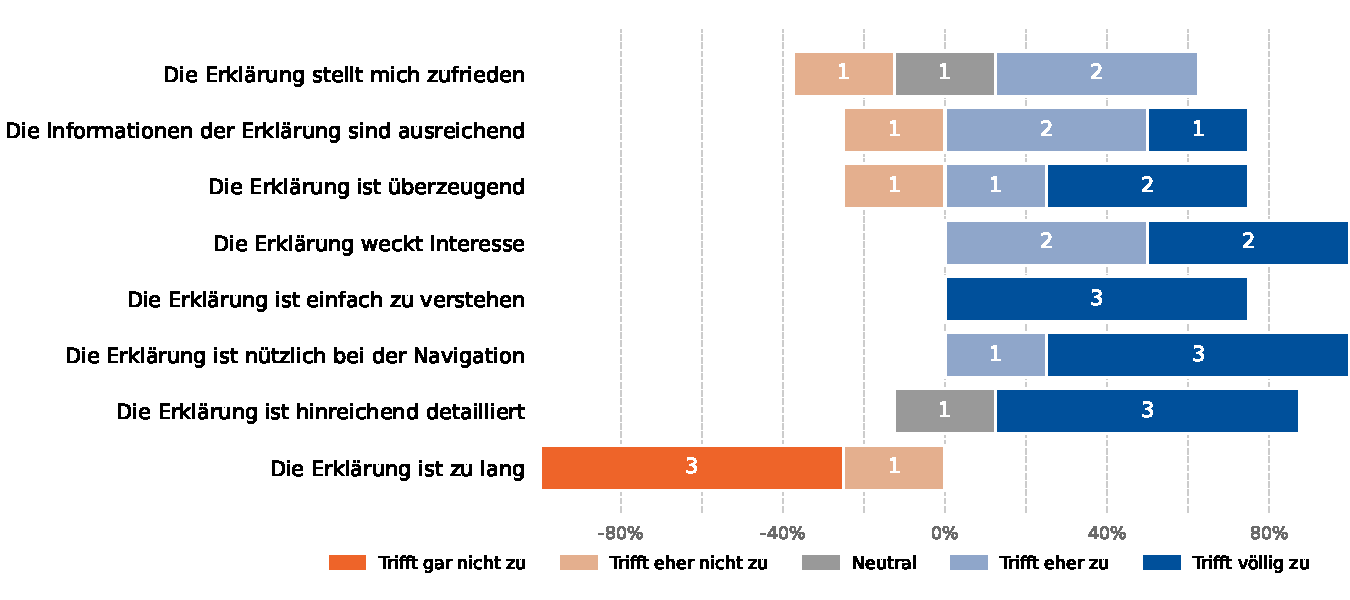
\includegraphics[width=\textwidth]{contents/06_model_evaluation/02_evaluation/res/qualitativeFeedback-04_position_accuracy_content.pdf}
    \caption{Subjektive Einschätzung des Inhalts für die Erklärung zu Positionsungenauigkeiten}
    \label{fig:04_position_accuracy_content}
\end{figure}

\subsubsection{Gestaltung der Erklärungen}

Neben der durchgeführten Analyse der verschiedenen Qualitätsmerkmale gab es außerdem vereinzelt Rückmeldungen zur \textit{Presentation} der Erklärungen.

Für die Erklärung des kollaborativen Routings wurde vorgeschlagen, dass die Erklärung mehr mit Grafiken arbeiten sollte, um den Algorithmus zu erklären.
% Das im Anschluss verlinkte Video würde das Kernthema mit wenigen Grafiken sehr gut zusammenfassen und verständlich machen.

Positiv wurden die Sprachansagen, die die Erklärung zum Verkehrsfluss und zur ungenauen Positionierung begleiten von mehreren Teilnehmern des Quasi-Experiments hervorgehoben. Diese würden explizit bei der Navigation im Auto sehr hilfreich sein, da sie nicht immer auf das Smartphone gucken würden.

